\section{The ATLAS Detector}%
\label{sec:atlas}

The ATLAS detector~\cite{PERF-2007-01}, shown in
\Cref{fig:atlas_detector_overview}, is a cylindrical particle detector
surrounding the LHC beamline at one of the IPs. The detector covers most of the
solid angle around the IP to ensure that all detectible particles from
collisions can be observed. The central part of the ATLAS detector is referred
to as the \emph{barrel}, while the two sections covering solid angles close to
the LHC beamline are referred to as the \emph{endcaps}. Different layers of
detector technologies are concentrically arranged around the IP that, in
conjunction, allow to detect and identify different types of particles, enabling
an almost full interpretation of collision events.

\begin{figure}[htbp]
  \centering

  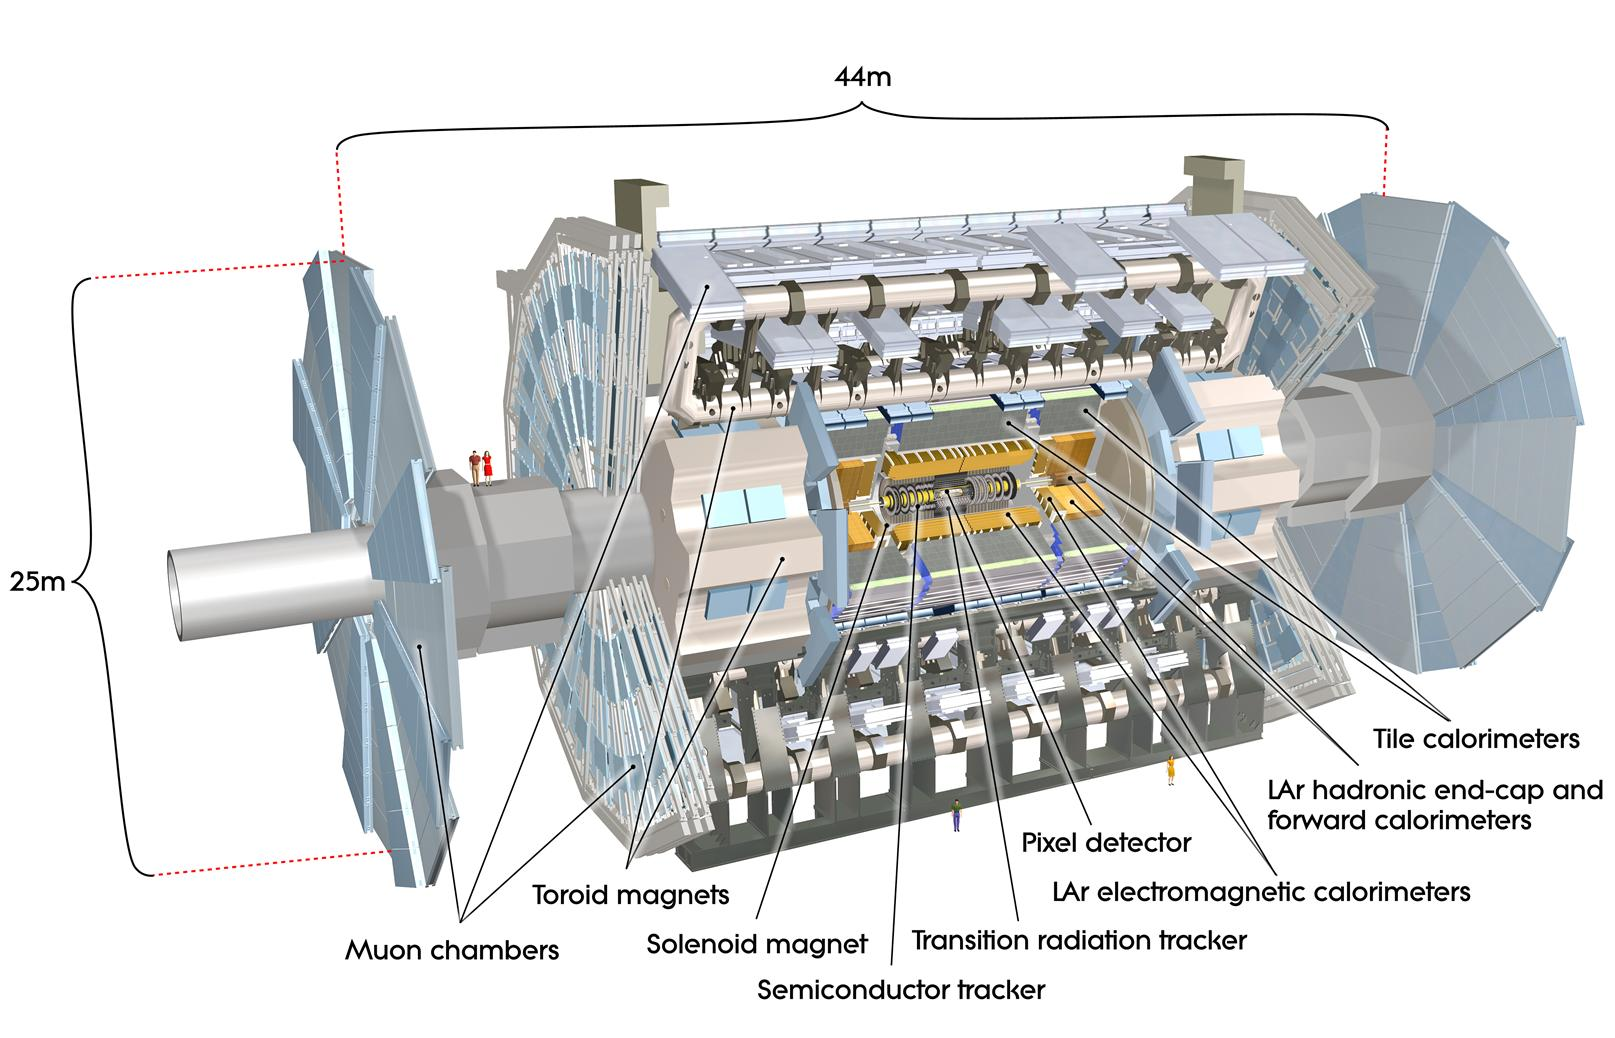
\includegraphics[width=0.76\textwidth]{atlas/atlas_overview}

  \caption{Overview of the ATLAS detector. Image taken from
    Ref.~\cite{Pequenao:1095924}.}%
  \label{fig:atlas_detector_overview}
\end{figure}

The ATLAS experiment uses a right-handed cartesian coordinate system with the
origin being located in the centre of the detector at the nominal IP. The axes
of the coordinate system are given as follows: the $x$-axis points to the centre
of the LHC, the $y$-axis points upwards, and the $z$-axis points along the LHC
beamline. The plane spanned by the $x$- and $y$-axes is referred to as the
transverse plane. A spherical coordinate system is used to specify directions in
three-dimensional space. The azimuthal angle, $\phi$, of this coordinate system
is defined as the angle in the transverse plane measured with respect to the
$x$-axis, and the polar angle, $\theta$, being the angle with respect to the
$z$-axis. With these coordinate systems, transverse momenta and energies are
defined as $\pT = \sqrt{p_x^2 + p_y^2} = p \sin\theta$ and $\ET = E \sin\theta$,
respectively. At hadron colliders, the polar angle is frequently given in terms
of the pseudorapidity $\eta$, which is defined as
\begin{align*}
  \eta = - \ln\tan\left( \frac{\theta}{2} \right) \,\text{.}
\end{align*}
Similarly, the angular separation between two particles is defined as
\begin{align*}
  \Delta R = \sqrt{\Delta \eta^2 + \Delta \phi^2} = \sqrt{(\eta_2 - \eta_1)^2 +
  (\phi_2 - \phi_1)^2} \,\text{,}
\end{align*}\todo{hold up. $\Delta \phi$ is not correct.}
where $\eta_1$ and $\eta_2$ are the pseudorapidities and $\phi_1$ and $\phi_2$
the azimuthal angle of both particles, respectively.

The main components of the ATLAS detector, going from the IP outwards, are the
\emph{Inner Detector} (ID) used for measuring the trajectories of charged
particles, the \emph{Calorimeters} used to destructively measure the energy of
most charged and neutral particles, and the \emph{Muon Spectrometer} (MS) used
to measure the trajectories of muons that can pass the calorimeters. Particles
in the ID are bent in the transverse plane due to a magnetic
field\todo{\SI{2}{\tesla}} pointing along the $z$-axis that is produced by a
superconducting solenoid surrounding the ID.  The MS is surrounded by a
superconducting toroid magnets that bend the trajectories of muons in or against
the $z$-direction. The bending of charged particle trajectories in the ID and MS
allows to determine the sign of the electric charge and momentum of
particles. The following sections summarise the most important parts of the
ATLAS detector.


\subsection{The Inner Detector}

The ID, depicted in \Cref{fig:atlas_inner_detector}, is the innermost part of
the ATLAS detector. It performs non-destructive measurements of the trajectories
of charged particles within $|\eta| < 2.5$ by measuring the points where charged
particles cross active detector layers. The measurment of several points on the
trajectory, and the known magnetic field in the ID, allows to reconstruct the
trajectory of the particle. The reconstructed trajectory is referred to as the
\emph{charged particle track} and sometimes abbreviated as \emph{track}. The
precise measurement of charged particle tracks is important to reconstruct the
primary vertex (PV) of the hard interaction with high spatial resolution,
allowing to remove tracks from pile-up which are typically displaced from the PV
along the $z$-axis. Moreover, the accurate reconstruction of secondary vertices,
i.e.\ displaced vertices originating from decays of unstable particles produced
in the hard interaction, is crucial to identify jets originating from
$b$-quarks.% which hinges on the precision of the track
% reconstruction in the ID.

\begin{figure}[htbp]

  \begin{subfigure}[b]{0.55\textwidth}
    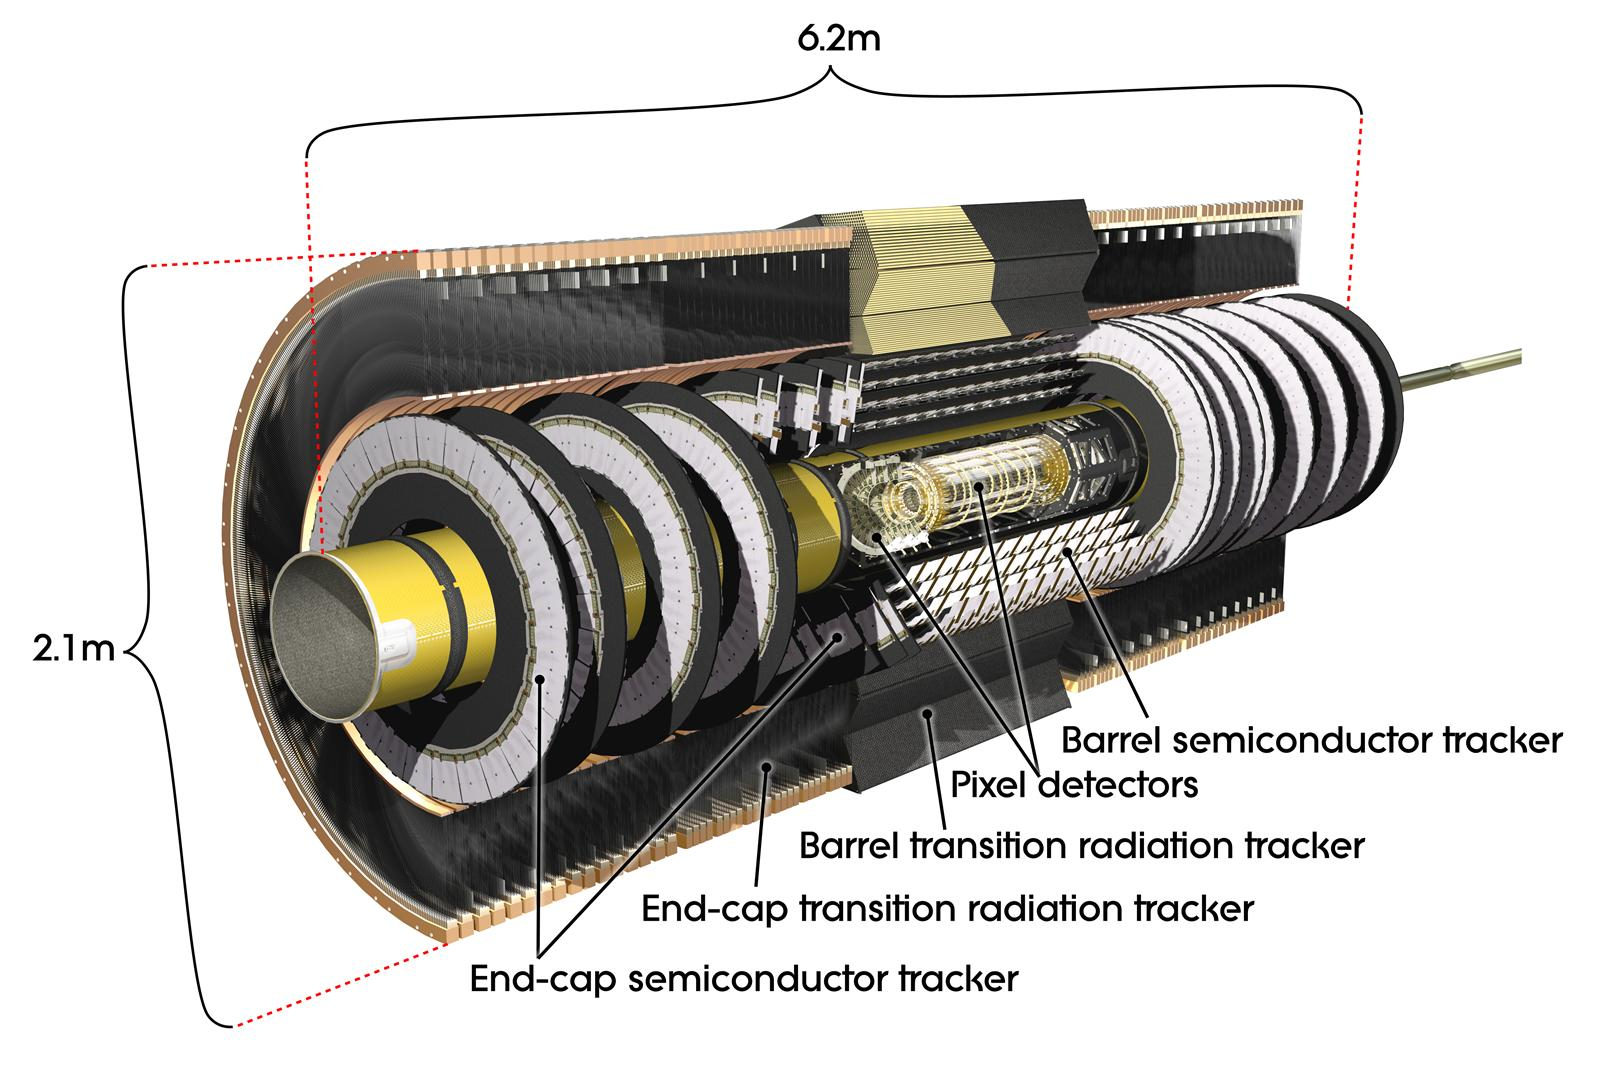
\includegraphics[width=\textwidth]{atlas/atlas_indet_1}%
    \subcaption{}
  \end{subfigure}\hfill%
  \begin{subfigure}[b]{0.45\textwidth}
    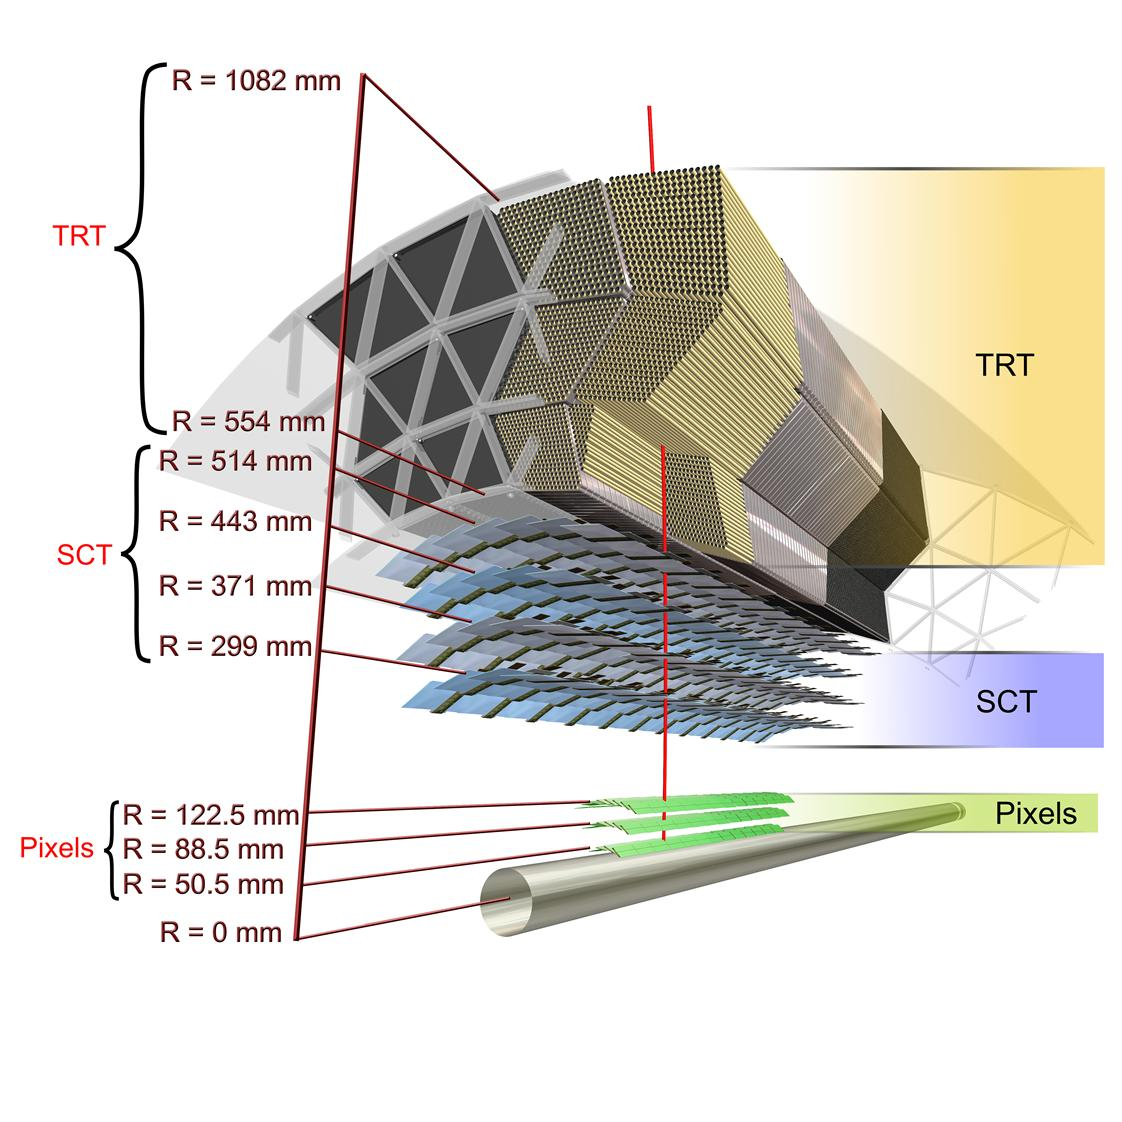
\includegraphics[width=\textwidth, trim=0 2.5cm 0 1cm,
    clip]{atlas/atlas_indet_2}%
    \subcaption{}%
    \label{fig:indet_barrel}
  \end{subfigure}

  \caption{Schematic view of the ID including the two endcaps (a). A zoomed in
    view of the barrel region of the ID (b). The Insertable B-Layer (IBL), which
    was introduced into the ATLAS detector after Run~1 of the LHC, is not
    displayed. The IBL is located closest to the beampipe at a radius of
    $r = \SI{33.5}{\milli\metre}$~\cite{ATLAS-TDR-19,PIX-2018-001}. Images taken
    from Ref.~\cite{Pequenao:1095926}.}%
  \label{fig:atlas_inner_detector}
\end{figure}

The requirements on the tracking system vary with the distance from the IP.
Closest to the IP, tracking detectors with high-granularity are required for the
reconstruction of primary and secondary vertices that can operate in a
high-radiation environment. At larger distances, the particle flux is
significantly reduced and the requirements on the spatial resolution relaxed.
Therefore, different detector technologies are used to cover the needs of the
tracking system in a cost-effective manner.

% Pixel
The ID subsystem closest to the beampipe are the pixel detectors located at
distances of \SIrange{33.5}{122.5}{\milli\metre} from the beamline in the barrel
region of the ATLAS detector (cf.\ \Cref{fig:atlas_inner_detector}). The pixel
detectors are based on semiconductor technology with an active detector area
that is segmented into a grid of rectangular elements, referred to as
pixels. These pixels have size of \SI{50}{\micro\metre} in the transverse
direction and \SIrange{250}{400}{\micro\metre} along the
beamline~\cite{PERF-2007-01,PIX-2018-001}. A charged particle traversing the
pixel detector ionises the active detector material leading to the deposition of
electric charge in nearby pixels. The charged deposited in individual pixels can
be read out to determine the point where the particle crossed the detector
layer. The pixel detectors are arranged in four layers concentric with the
beamline in the barrel region and three disks per endcap region. Particles
produced at the IP typically traverse four layers of pixel detectors within the
acceptance of $|\eta| < 2.5$ of the tracking system.

% SCT
The pixel detector is surrounded by the \emph{Semiconductor Tracker} (SCT)
covering radii of \SIrange{299}{514}{\milli\metre} from the beamline in the
barrel region (cf.\ \Cref{fig:atlas_inner_detector}). Similar to the pixel
detector, the SCT is based on semiconductor detector technology, however, the
active detector area is segmented in long but thin strips (microstrips) with a
pitch between strips of about \SI{80}{\micro\metre}~\cite{PERF-2007-01}. A
single microstrip detector layer only provides an accurate position measurement
in the plane perpendicular to the strips. Therefore, SCT modules consist of two
layers of microstrips which are tilted by a small angle to resolve the ambiguity
in the direction parallel to the strips. The SCT is arranged in four layers in
the barrel and nine disks in the endcap region, yielding at least four
measurements for tracks within the acceptance of the tracking
system~\cite{PERF-2007-01}.

% TRT
The \emph{Transition Radiation Tracker} (TRT) is the final layer of the ID
covering radii of \SIrange{554}{1082}{\milli\metre} (cf.\
\Cref{fig:atlas_inner_detector}), however, with reduced acceptance of
$|\eta| < 2.0$ compared to the semiconductor-based trackers.

The TRT consists of drift tube


Gaseous tracking detector TRT ($|\eta| < 2.0$) and electron identification
information.


\subsection{Calorimeters}

\begin{figure}[htbp]
  \centering

  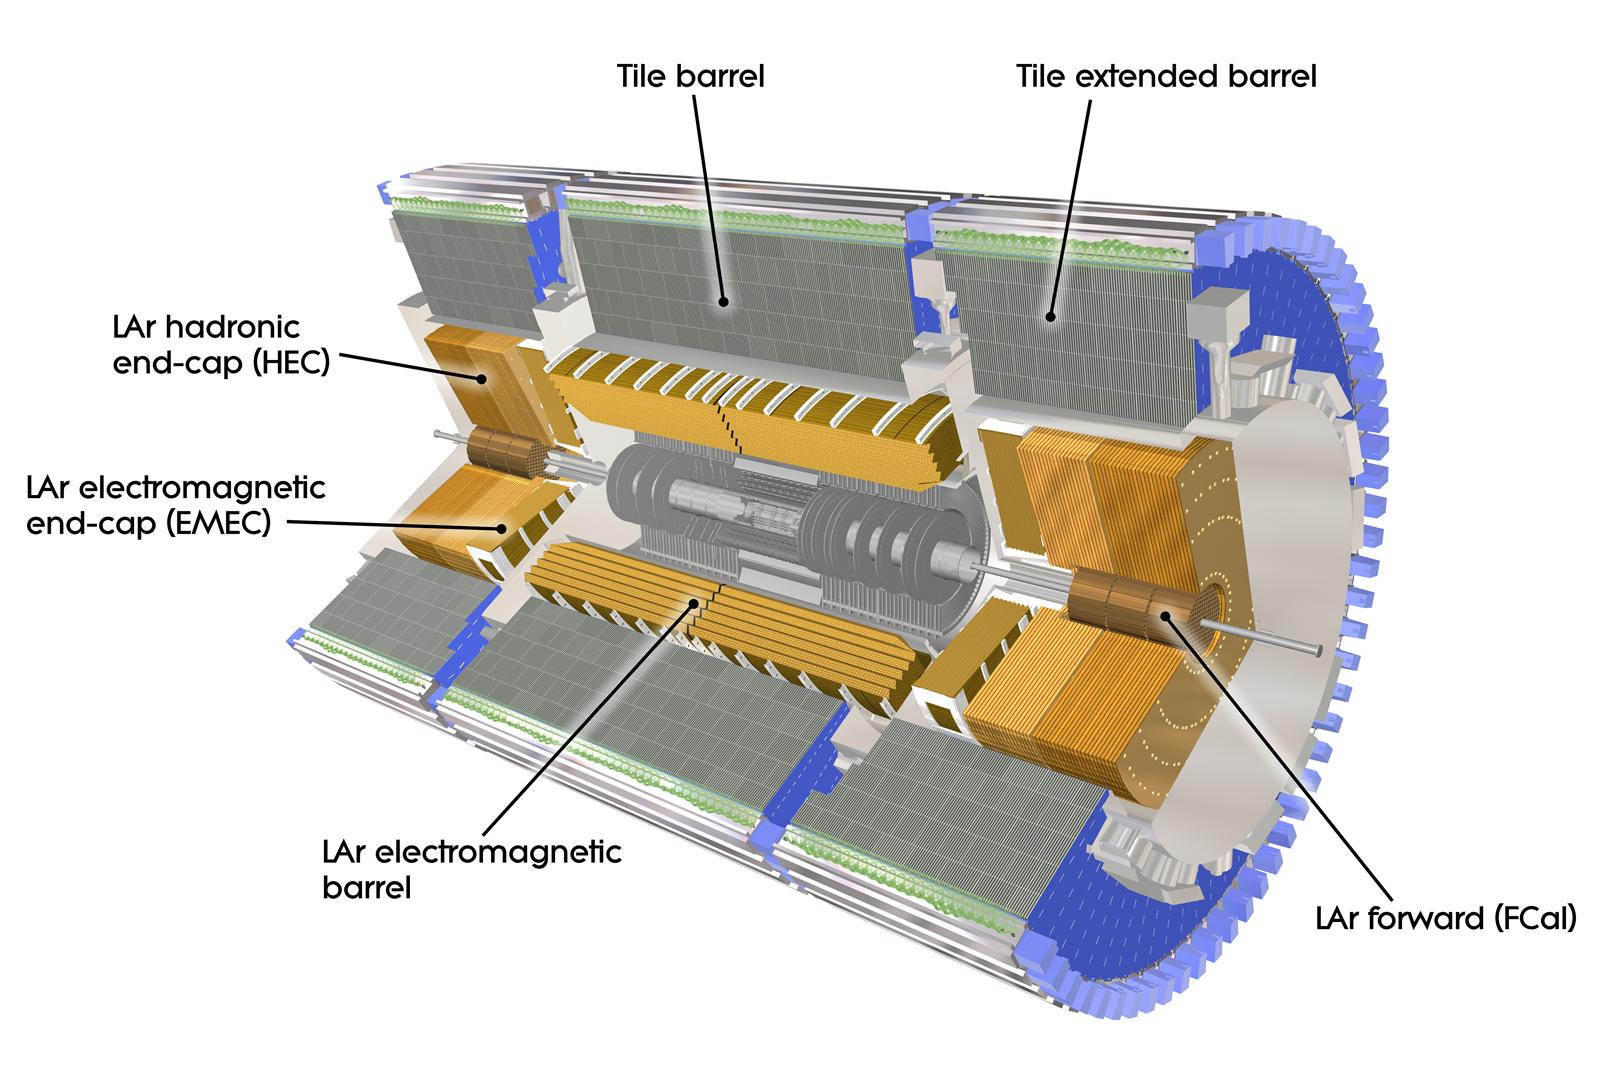
\includegraphics[width=0.65\textwidth]{atlas/atlas_calo}

  \caption{Calorimeters. Image taken from Ref.~\cite{Pequenao:1095927}.}%
  \label{fig:atlas_calorimeters}
\end{figure}


\subsection{Muon Spectrometer}

\begin{figure}[htbp]
  \centering

  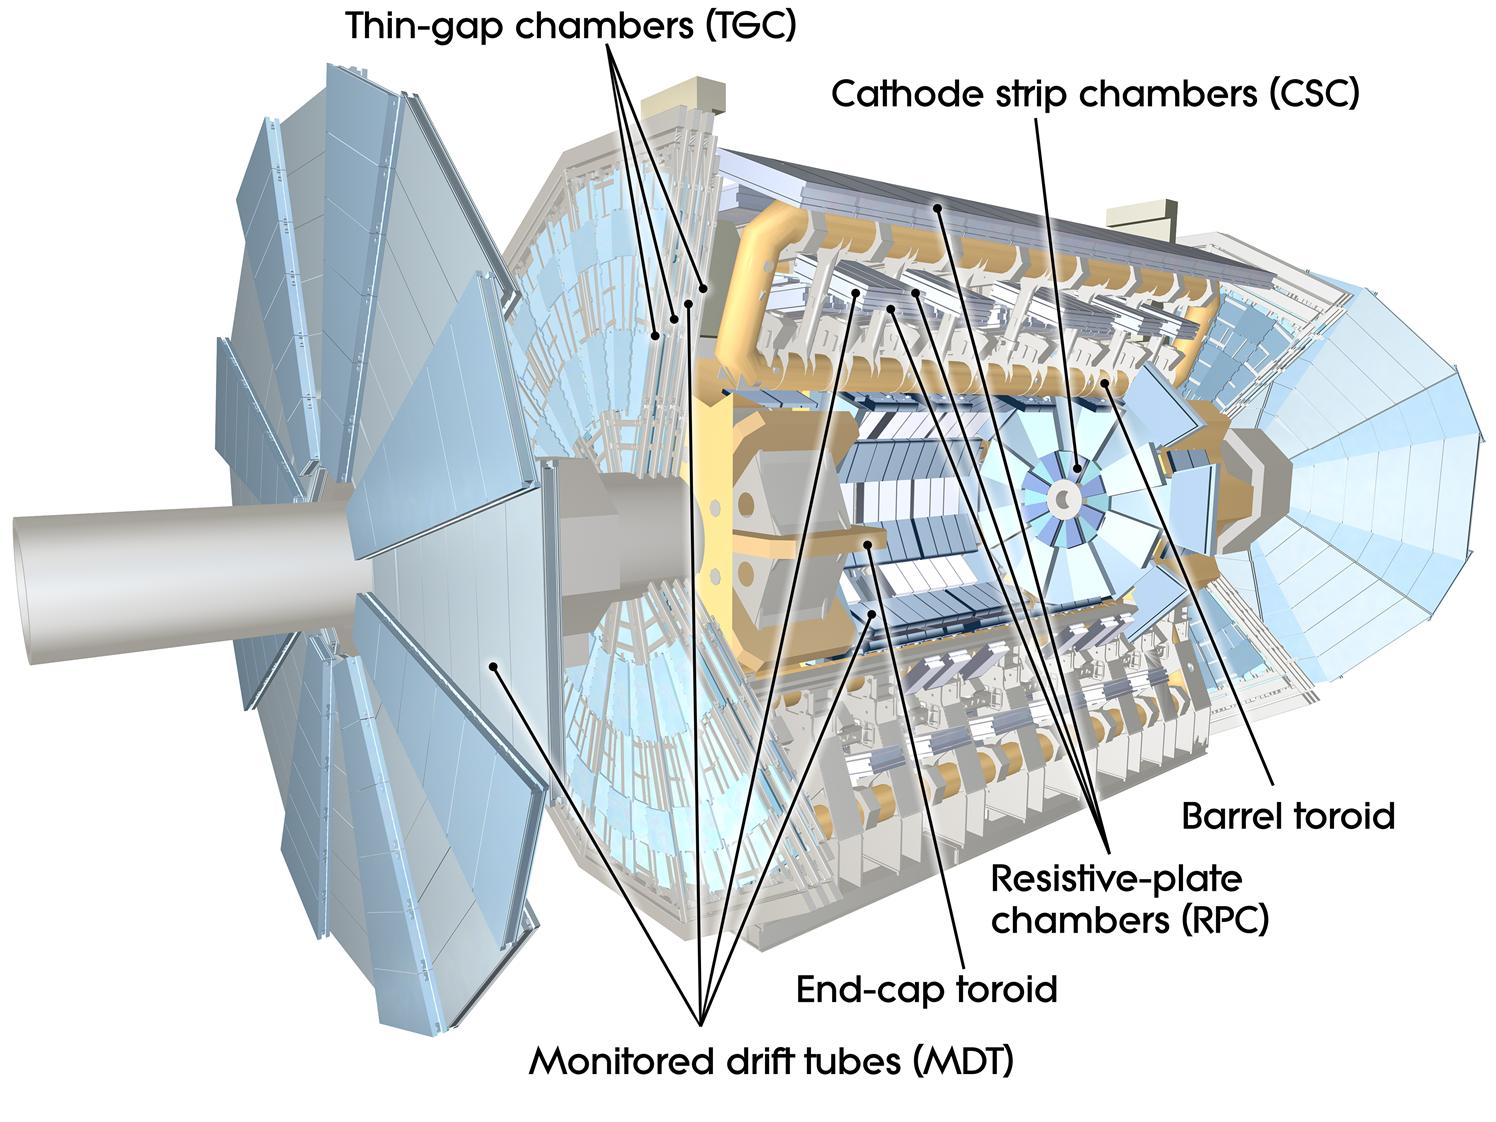
\includegraphics[width=0.65\textwidth]{atlas/atlas_muon}

  \caption{Muon subsystems. Image taken from Ref.~\cite{Pequenao:1095929}.}%
  \label{fig:atlas_muon_system}

  \todo[inline]{Is this really needed?}
\end{figure}

\subsection{The ATLAS Trigger System}

%%% Local Variables:
%%% mode: latex
%%% TeX-master: "../../phd_thesis"
%%% End:
